%% Beginning of file 'sample631.tex'
%%
%% Modified 2021 March
%%
%% This is a sample manuscript marked up using the
%% AASTeX v6.31 LaTeX 2e macros.
%%
%% AASTeX is now based on Alexey Vikhlinin's emulateapj.cls 
%% (Copyright 2000-2015).  See the classfile for details.

%% AASTeX requires revtex4-1.cls and other external packages such as
%% latexsym, graphicx, amssymb, longtable, and epsf.  Note that as of 
%% Oct 2020, APS now uses revtex4.2e for its journals but remember that 
%% AASTeX v6+ still uses v4.1. All of these external packages should 
%% already be present in the modern TeX distributions but not always.
%% For example, revtex4.1 seems to be missing in the linux version of
%% TexLive 2020. One should be able to get all packages from www.ctan.org.
%% In particular, revtex v4.1 can be found at 
%% https://www.ctan.org/pkg/revtex4-1.

%% The first piece of markup in an AASTeX v6.x document is the \documentclass
%% command. LaTeX will ignore any data that comes before this command. The 
%% documentclass can take an optional argument to modify the output style.
%% The command below calls the preprint style which will produce a tightly 
%% typeset, one-column, single-spaced document.  It is the default and thus
%% does not need to be explicitly stated.
%%
%% using aastex version 6.3
%\documentclass[linenumbers]{aastex631}
\documentclass[twocolumn]{aastex631}

\usepackage{amsmath}
\usepackage{hyperref}
\usepackage{booktabs}
\usepackage{longtable}
\usepackage{savesym}
\savesymbol{tablenum}
\usepackage{placeins}
\usepackage{siunitx}
\usepackage[T1]{tipa}

\usepackage{threeparttable}
\restoresymbol{SIX}{tablenum}
\sisetup{
    %binary-units,
    range-phrase=\text{--},
    range-units=single,
    separate-uncertainty=true,
    retain-explicit-plus,
    % exponent-mode=scientific,
    % table-format=1e1,
    % print-zero-exponent=true, 
    % print-unity-mantissa=false
    }
\DeclareSIUnit{\parsec}{pc}
\DeclareSIUnit{\jansky}{Jy}
\DeclareSIUnit{\dmunit}{pc cm^{-3}}

\DeclareTextFontCommand{\textipa}{%
  \fontfamily{cmss}\tipaencoding
}
\renewenvironment{IPA}{\fontfamily{cmss}\tipaencoding}{}


\newcommand{\kkoname}{k'ni\textipa{P}atn k'l$\left._\mathrm{\smile}\right.$stk'masqt}

\newcommand{\muhost}{\mu_\textrm{host}}
\newcommand{\remove}[1]{\textcolor{green}{#1}}
\newcommand{\sighost}{\sigma_\textrm{host}}
\newcommand{\dmh}{\ensuremath{{\rm DM}_\textrm{h}}}
\newcommand{\pox}{\ensuremath{P(O|x)}}
\newcommand{\dmcosmic}{\ensuremath{{\rm DM}_{\rm cosmic}}}
%% Reintroduced the \received and \accepted commands from AASTeX v5.2
\received{\today}%
\revised{\today}
\accepted{\today}

%% Command to document which AAS Journal the manuscript was submitted to.
%% Adds "Submitted to " the argument.
\submitjournal{ApJS}

%% For manuscript that include authors in collaborations, AASTeX v6.31
%% builds on the \collaboration command to allow greater freedom to 
%% keep the traditional author+affiliation information but only show
%% subsets. The \collaboration command now must appear AFTER the group
%% of authors in the collaboration and it takes TWO arguments. The last
%% is still the collaboration identifier. The text given in this
%% argument is what will be shown in the manuscript. The first argument
%% is the number of author above the \collaboration command to show with
%% the collaboration text. If there are authors that are not part of any
%% collaboration the \nocollaboration command is used. This command takes
%% one argument which is also the number of authors above to show. A
%% dashed line is shown to indicate no collaboration. This example manuscript
%% shows how these commands work to display specific set of authors 
%% on the front page.
%%
%% For manuscript without any need to use \collaboration the 
%% \AuthorCollaborationLimit command from v6.2 can still be used to 
%% show a subset of authors.
%
%\AuthorCollaborationLimit=2
%
%% will only show Schwarz & Muench on the front page of the manuscript
%% (assuming the \collaboration and \nocollaboration commands are
%% commented out).
%%
%% Note that all of the author will be shown in the published article.
%% This feature is meant to be used prior to acceptance to make the
%% front end of a long author article more manageable. Please do not use
%% this functionality for manuscripts with less than 20 authors. Conversely,
%% please do use this when the number of authors exceeds 40.
%%
%% Use \allauthors at the manuscript end to show the full author list.
%% This command should only be used with \AuthorCollaborationLimit is used.

%% The following command can be used to set the latex table counters.  It
%% is needed in this document because it uses a mix of latex tabular and
%% AASTeX deluxetables.  In general it should not be needed.
%\setcounter{table}{1}

%%%%%%%%%%%%%%%%%%%%%%%%%%%%%%%%%%%%%%%%%%%%%%%%%%%%%%%%%%%%%%%%%%%%%%%%%%%%%%%%
%%
%% The following section outlines numerous optional output that
%% can be displayed in the front matter or as running meta-data.
%%
%% If you wish, you may supply running head information, although
%% this information may be modified by the editorial offices.
\shorttitle{Host DM}
\shortauthors{CHIME/FRB Collaboration et al.}
%%
%% You can add a light gray and diagonal water-mark to the first page 
%% with this command:
%% \watermark{text}
%% where "text", e.g. DRAFT, is the text to appear.  If the text is 
%% long you can control the water-mark size with:
%% \setwatermarkfontsize{dimension}
%% where dimension is any recognized LaTeX dimension, e.g. pt, in, etc.
%%
%%%%%%%%%%%%%%%%%%%%%%%%%%%%%%%%%%%%%%%%%%%%%%%%%%%%%%%%%%%%%%%%%%%%%%%%%%%%%%%%
\graphicspath{{./}{figures/}}
%% This is the end of the preamble.  Indicate the beginning of the
%% manuscript itself with \begin{document}.

\begin{document}

\title{Cosmology-insensitive constraints on the circumgalactic medium of fast radio burst hosts}

%% LaTeX will automatically break titles if they run longer than
%% one line. However, you may use \\ to force a line break if
%% you desire. In v6.31 you can include a footnote in the title.

%% A significant change from earlier AASTEX versions is in the structure for 
%% calling author and affiliations. The change was necessary to implement 
%% auto-indexing of affiliations which prior was a manual process that could 
%% easily be tedious in large author manuscripts.
%%
%% The \author command is the same as before except it now takes an optional
%% argument which is the 16 digit ORCID. The syntax is:
%%
%% This will hyperlink the author name to the author's ORCID page. Note that
%% during compilation, LaTeX will do some limited checking of the format of
%% the ID to make sure it is valid. If the "orcid-ID.png" image file is 
%% present or in the LaTeX pathway, the OrcID icon will appear next to
%% the authors name.
%%
%% Use \affiliation for affiliation information. The old \affil is now aliased
%% to \affiliation. AASTeX v6.31 will automatically index these in the header.
%% When a duplicate is found its index will be the same as its previous entry.
%%
%% Note that \altaffilmark and \altaffiltext have been removed and thus 
%% can not be used to document secondary affiliations. If they are used latex
%% will issue a specific error message and quit. Please use multiple 
%% \affiliation calls for to document more than one affiliation.
%%
%% The new \altaffiliation can be used to indicate some secondary information
%% such as fellowships. This command produces a non-numeric footnote that is
%% set away from the numeric \affiliation footnotes.  NOTE that if an
%% \altaffiliation command is used it must come BEFORE the \affiliation call,
%% right after the \author command, in order to place the footnotes in
%% the proper location.
%%
%% Use \email to set provide email addresses. Each \email will appear on its
%% own line so you can put multiple email address in one \email call. A new
%% \correspondingauthor command is available in V6.31 to identify the
%% corresponding author of the manuscript. It is the author's responsibility
%% to make sure this name is also in the author list.
%%
%% While authors can be grouped inside the same \author and \affiliation
%% commands it is better to have a single author for each. This allows for
%% one to exploit all the new benefits and should make book-keeping easier.
%%
%% If done correctly the peer review system will be able to
%% automatically put the author and affiliation information from the manuscript
%% and save the corresponding author the trouble of entering it by hand.

\correspondingauthor{CHIME}%Calvin Leung}
\email{calvin\_leung@berkeley.edu}


\author[0000-0002-4209-7408]{C.~Leung}
\affiliation{UC Berkeley}

\collaboration{99}{(CHIME/FRB Collaboration)}

%% Note that the \and command from previous versions of AASTeX is now
%% depreciated in this version as it is no longer necessary. AASTeX 
%% automatically takes care of all commas and "and"s between authors names.

%% AASTeX 6.31 has the new \collaboration and \nocollaboration commands to
%% provide the collaboration status of a group of authors. These commands 
%% can be used either before or after the list of corresponding authors. The
%% argument for \collaboration is the collaboration identifier. Authors are
%% encouraged to surround collaboration identifiers with ()s. The 
%% \nocollaboration command takes no argument and exists to indicate that
%% the nearby authors are not part of surrounding collaborations.

%% Mark off the abstract in the ``abstract'' environment. 
\begin{abstract}
Low-redshift host galaxies are crucial components of FRB cosmology, providing the tightest and most robust constraints on the circumgalactic medium of FRB hosts via the inferred host component of the dispersion measure (DM) budget. We infer the mean and standard deviation of the host contribution for non-dwarf host galaxies ($M_r > -17$) to be $104\pm 16$ and $113\pm12$ pc cm$^{-3}$; this characterization is the most precise to date and is insensitive to galactic feedback models by virtue of the low redshift ($z \sim 0.1$) of our sample. We show that our measurement is insensitive to the IGM and cosmological contributions, and present evidence for a weak dependence of \dmh\ over a range of $\approx 100$ in stellar light, which in turn is tightly correlated to halo mass. Comparing our data to predictions from the CAMELS simulations, we rule out models which predict large ($\sim 200$ pc cm$^{-3}$) mean host contributions.
\end{abstract}
\keywords{Very long baseline interferometry (1769), Radio transient sources (2008)}

\section{Introduction}\label{sec:intro}
Long before the first repeating fast radio burst (FRB) was localized to a cosmologically-distant host galaxy~\citep{chatterjee2017direct,tendulkar2017host}, the immense potential of FRBs as cosmological probes of the cosmic baryons was recognized~\citep{mcquinn2014locating}.

Previous observational characterization of the host galaxies of FRBs has followed in the footsteps of the gamma-ray burst (GRB) community~\citep{bloom2002observed,fong2022comprehensive} by focusing primarily on their role in constraining FRB progenitors. In this paper we use the low-redshift catalog of FRBs, presented in a companion work, in order to study the contribution of the host galaxy to the dispersion measure budget: a crucial part of virtually every proposed application of FRBs as cosmological probes.

One of the earliest studies of FRB host galaxies used five FRB host galaxies localized by the Australian Square Kilometre Array Pathfinder~\citep{macquart2020census} to locate the missing baryons to the intergalactic medium (IGM). That landmark result established that the host contribution to the dispersion measure budget was on average dominated by that of the intergalactic medium, establishing what FRB astronomers refer to as the ``Macquart relation''. Populations analyses on a small sample of hosts allowed for cosmological constraints~\citep{james2022measurement} to follow shortly thereafter.

Recently, the Deep Synoptic Array has detected tens of FRBs and localized them to their host galaxies~\citep{connor2024gas}, with redshifts ranging from  $z = 0.04$ to $1.3$. Partitions of the cosmic baryon budget followed, using the redshift evolution of the IGM contribution to the DM budget to disentangle it from the host galaxy contribution.

However, a study dedicated to FRB host galaxies in the context of FRBs as probes remains unexplored, even though the distribution of the host galaxy DM contribution (hereafter, \dmh) is crucial to virtually all attempts to forward model FRB dispersion measures as probes of ionized gas. For instance, through analyses of the joint probability distribution of extragalactic DM as a function of redshift~\citep{james2021z}, FRBs have been touted as excellent probes of the baryon density $\Omega_b$, the ionization state of the intergalactic medium, and even the Hubble constant; yet these quantities are often degenerate with host galaxy properties in models ~\citep[e.g. Fig. 9 of][]{james2022measurement}. Two-point cross-correlation analyses are also possible; yet these cross-correlation analyses depends on having low levels of contamination from other line-of-sight contributions including residual contamination from the Milky Way, the host galaxy ISM/halo, and circumsource media, e.g., a star-forming region or an HII region~\citep{mcquinn2014locating,rafiei_ravandi2021chime,2019arXiv190102418M}.

Individual DM budgets have been observed to both undershoot ~\citep[FRB 20220319B; see][]{ravi2023deep} and overshoot expectations due to an insufficiently-modeled sightline~\citep[e.g. FRB 20190520A][]{niu2021repeating,lee2023frb}. With every new FRB, observers are motivated to dissect in great detail~\citep{2024arXiv240200505K} the origin of the DM excess after subtracting DM$_\text{cosmic}$: is the remainder dominated by a dense circum-source medium, or could it possibly originate from gas along the line of sight?

At $z \gtrsim 0.2$ this question is difficult to answer because the contribution of large-scale structure to the DM budget -- the overdensities/underdensities relative to $\langle \textrm{DM}_\text{cosmic}\rangle$ -- dominates over smaller-scale contributions from e.g. the host galaxy and circum-source medium. While estimates are highly uncertain,~\citet{walker2024dispersion} estimate an RMS fluctuation in DM$_\textrm{cosmic}$ of $\gtrsim 100$ pc cm$^{-3}$ -- roughly the size of the mean host contribution -- beyond $z = 0.2$. Though notable exceptions exist, this is enough noise to swamp the DM contribution from most circum-source media and Milky Way-like electron disks at most inclination angles. 

At lower redshifts, this question is more tractable since the mean cosmic contribution %and the large-scale structure contributions 
to the DM budget is low ($\lesssim 100$ \,pc~cm$^{-3}$). At a low redshift and above a certain DM threshold ($z < 0.2$, DM$_{eg} \gtrsim 200$ pc cm$^{-3}$), the discrete structures responsible for DM excesses and deficits may be identifiable in archival surveys with little or no casework. This is because the probability of encountering multiple line-of-sight structures is $\ll 1$ for halo masses exceeding $>10^{12} M_\odot$~\citep[Fig.~1 of][]{mcquinn2014locating}, whereas most FRB hosts originate in galaxies with stellar masses of $10^{10-11} M_{\odot}$, making the host galaxy the dominant contributor to the DM budget after subtracting the average cosmic contribution. Fig.~\ref{fig:host_dm} summarizes our efforts to identify sources of large DM excesses in this pristine regime where the host galaxy contribution may be measured with little line-of-sight contamination.

In \S~\ref{sec:dmh} we describe our measurement of the host galaxy contribution to the DM budget. In \S~\ref{sec:sample} we describe various critical subsamples of FRBs which we identify to disentangle instrumental selection biases and to assess impact of intervening gas. We analyze the sensitivity of our measurement to changes to cosmology and the baryon budget in \S~\ref{sec:sensitivity}. Finally in \S~\ref{sec:where} we discuss the source of the host DM, concluding that it probably originates from the host halo. This is consistent with a picture of gas being expelled from haloes.

All quantities in this work are calculated using the \textit{Planck} cosmology for a flat $\Lambda$CDM universe of  $H_0 = 67.7~\mathrm{km~s}^{-1}~\mathrm{Mpc}^{-1}$, $\Omega_m=0.31$ and $\Omega_\Lambda = 0.69$ \citep{collaboration2020planck}. 

 As detailed in \S\ref{sec:sample}, the vast majority of cases for $\dmh > 200$ pc cm$^{-3}$, an edge-on galaxy or line-of-sight structure can be identified as a plausible source of the DM excess, but we reserve detailed characterization to future work.

\section{Sample Selection}\label{sec:dmh}
We statistically characterize the $\dmh$ distribution at low redshifts, using our sample of low-redshift hosts to significantly expand the low-redshift dataset as seen in
Fig.~\ref{fig:macquart}. We have compiled the vast majority of FRBs with secure redshifts and publicly-available photometry detected to date, using the host galaxies in this paper to assemble a combined sample of 49 host galaxies at $z < 0.2$ (Fig.~\ref{fig:macquart}). This allows us to make the most precise and feedback-insensitive measurement of the distribution of \dmh (see Eq.~\ref{eq:dmh_definition}).

In principle, \dmh\ is contaminated by contributions from all line-of-sight structures, but at low redshifts it is likely to be dominated by contributions from the host galaxies of FRBs. It is often modeled statistically as a log-normal distribution with a mean $\muhost$ and width $\sighost$. This parametrization is ubiquitous \citep[e.g.,][]{macquart2020census,james2021z,baptista2024measuring} yet lacks physical justification and has obvious drawbacks. For instance, in this parameterization the RMS scatter in $\dmh$ cannot be decoupled from the heaviness of its tail, i.e. the skew.

To improve on this, we directly measure the first four moments (i.e., the mean, width, skew, and excess kurtosis) of the $\dmh$ distribution. Effects such as scattering and propagation through the inclined disks of FRB host galaxies will modify the moments of the $\dmh$ distribution; in the future the locations of FRBs within their host galaxies could potentially be disentangled by their distinct imprints on the moments of the $\dmh$ distribution.

We first summarize all available data on the $\dmh$ distribution in Figs.~\ref{fig:macquart} and~\ref{fig:host_dm}. Next, we perform a redshift cut ($z < 0.2$), and exclude from our analysis non-luminous ($M_r > -17$) and dwarf hosts \citep[FRB 20121102A, FRB 20190520B, FRB 20210117A; FRB][]{bhandari2023nonrepeating,hewitt2024repeating}. These sources are not representative from the population of detected FRBs; on the basis of the high specific star formation rates of their hosts and persistent radio source counterparts their progenitors may be produced by a formation channel distinct from that of FRBs from more massive galaxies. For this reason, our \dmh\ parameter estimates are valid only for FRBs with non-dwarf hosts over the aforementioned range of host stellar masses. Finally, we identify the following critical subsamples of FRBs within the remaining 49 FRBs:
\begin{enumerate} 
\item We separately consider FRBs (all from CHIME/FRB) for which the low total DM was crucial to making a host galaxy association because of the explicit selection bias on \dmh~\citep[8 bursts from ][]{bhardwaj2024host,michilli2023subarcminute,Ibik2024host}. Analyzing this sub-sample separately confirms that these bursts are drawn from the low-\dmh\ tail of the FRB population.
\item We also separately considerisolate galaxy cluster FRBs, since these have significant contamination from outside their host galaxy. These include FRB 20220914A and FRB 20220509G~\citep{connor2023deep}, FRB 20231206A (\S~\ref{sec:FRB20231206A}), FRB 20230203A (\S~\ref{sec:FRB20230203A}), and FRB 20231204A (\S~\ref{sec:FRB20231204A}). While we have not performed a complete search, we note that clusters account for a significant fraction of the largest outliers ($\dmh > 200$ pc cm$^{-3}$) observed in our sample, suggesting that we are complete to associated clusters whose foreground DM contribution exceeds this threshold.
\item We separately consider edge-on host galaxies, for which we report inclinations where available. These include FRB 20210603A \citep[$i \sim 83^\circ$; ][]{cassanelli2024fast}, FRB 20220207C \citep[$i \sim 74-80^\circ$;][]{law2024deep,bhardwaj2024selection}, and two FRBs from this work: FRB 20230203A ($i \sim 77-81^\circ$) and FRB 20231005A ($i \sim 81^\circ$), for which we apply the InclinationZoo estimator~\citep{kourkchi2020cosmicflows} to publicly-available SDSS and Pan-STARRS imaging, verifying that that measurements are robust between both images. Three remaining FRBs have no quantitative estimates readily available, but their host galaxies appear highly elongated in published images justifying their classification as edge-on: FRB 20231120A~\citep{2024arXiv240916964S}, and FRB 20240201A and FRB 20240310A from~\citet{shannon2024commensal}. 
\end{enumerate}

We then measure the first four moments of the $\dmh$ distribution using our full sample of $z < 0.2$ FRBs as well as the three aforementioned subsamples (low-DM, edge-on, and galaxy cluster FRBs). The four moments are defined in Eq.~\ref{eq:mean}-\ref{eq:kurt}. In all cases, each data point is weighted to account for errors in the NE2001 model and an RMS contribution from the cosmic web. In addition, we de-bias the kurtosis estimate (by subtracting 3) such that a Gaussian distribution of \dmh\ values has $\kappa_h = 0$. %$\sigma_\textrm{IGM}^2$ to the results of dispersion-measure ray tracing through the Illustris TNG simulation~\citep{walker2024dispersion}, but note that the small redshift range ($z < 0.2$) prevents us from disentangling our fitted parameter $S_h^2$ from $\sigma_\textrm{IGM}^2$, which adds 63.3 pc cm$^{-3}$ of RMS scatter at $z = 0.1$ and 105 pc cm$^{-3}$ at $z = 0.2$. 


\begin{align} 
\langle \dmh\rangle &= \dfrac{\sum_i w_i \dmh{}_{,i}}{\sum_i w_i} \label{eq:mean}\\
S_h^2 &= \dfrac{\sum_i w_i (\dmh{}_{,i} - M_h)^2}{\sum_i w_i}\label{eq:std} \\
\Gamma_h &= \dfrac{\sum_i w_i (\dmh{}_{,i} - M_h)^3}{S_h^{3}\sum_i w_i} \label{eq:skew}\\
\kappa_h &= \dfrac{\sum_i w_i (\dmh{}_{,i} - M_h)^4}{S_h^{4}\sum_i w_i} - 3.\label{eq:kurt}
\end{align}

The weights are defined to be $w_i \propto \sigma_i^{-2}$ with $$\sigma_i^2 = (0.2\text{DM}_\textrm{NE2001,i})^2 + (10~\text{pc cm}^{-3})^2 + \sigma_\textrm{cosmic}^{2}.$$ This formula accounts for 20\% uncertainties in the Milky Way disk model, a constant uncertainty in the MW halo model, and an RMS scatter in the cosmic dispersion measure originating from haloes as well as the IGM. We fix $\sigma_\textrm{cosmic} = 80~\text{pc cm}^{-3}$ in order to be roughly consistent with estimates from~\citet{walker2024dispersion}. While it is difficult to separate the RMS scatter in the IGM from $S_h$ we find that our results are insensitive to the particular value of $\sigma_\textrm{IGM}$ used, since this choice only affects the relative weighting of the data. Choosing $\sigma_\textrm{IGM} = 0$ shifts the final parameter estimates by at most $5\%$ of our quoted measurement uncertainty, which was estimated by bootstrapping each sample with replacement 4000 times. 

Our final parameter estimates for our full sample and various sub-samples are shown in Fig.~\ref{fig:mvsk} and Table~\ref{tab:mvsk}. Measurements from our full sample are the most precise ($\sim 10\%$) estimates to date and are insensitive to galactic feedback or a particular functional form of the distribution. In addition, measurements are performed independently for the low-DM, edge-on, and galaxy cluster subsamples. Finally, these three sets of FRBs are removed from the full sample in an attempt to define a ``clean'' subsample for cosmological measurements. In particular, we expect that relative to the full sample, $\langle\dmh\rangle$ for the ``clean'' subsample will be less biased, and that $S_h$ will be reduced. While each of these samples have very different $\dmh$, they roughly counterbalance each other in terms of the overall effect on $\dmh$. We see that $S_h$ is also largely unaffected by this change.


We can compare our measurements to existing measurements of the host galaxy contribution \citep{james2021z,shin2023inferring,connor2024gas} using analytical expressions which translate the log-normal distribution into non-log space. We compare only the mean, i.e. $\langle \dmh\rangle$ because of each methods' different assumptions. First, the number of bursts cannot be directly translated, since in global fitting analyses, low-redshift bursts constrain the mean host contribution, whereas high-redshift bursts mainly constrain the IGM. In addition, unlocalized and localized FRBs have vastly different constraining power.

The scatter and tail of the distribution cannot be directly compared either, since in those analyses, the RMS host galaxy contribution is divided into host-related and cosmic contributions using an assumed redshift dependence of the latter. In contrast, our measurement makes no assumptions about the redshift dependence but does not allow for the IGM and host contributions to $S_h$ to be separated.

We see no strong trend when binned by host luminosity, nor when dividing the sample by detection experiment; but sightlines with galaxy clusters and edge-on host galaxies, as well as FRBs selected on the basis of their total DM have significantly different values of $\langle\dmh\rangle$: a warning sign for attempts to simplistically model the host galaxy contribution. 

First, we split our sample based on the median $M_r$. The $\langle\dmh \rangle$ distribution for host galaxies within the ranges $-23 > M_r > -20.6$ and $-20.6 > M_r > -17$ differ by $\approx 30$ pc cm$^{-3}$, a $\sim 1\sigma$ effect.

Second, we find that relative to the parent sample (``All''), FRBs in groups, clusters and edge-on host galaxies have much higher values of $\langle \dmh\rangle$ ($> 100$ pc cm$^{-3}$) but similar values of $S_h$ to that of the parent sample. This implies that these systems will bias all cosmological analyses which are sensitive to $\langle\dmh\rangle$.

Third, we find that low-DM selected FRBs have a \dmh\ distribution with much lower mean and standard deviation from the others, implying they should be omitted from population-level cosmological analyses spanning a wide range of redshifts, unless accounted for in a model of the redshift evolution of $\langle\dmh\rangle$. 

Finally, we sub-divide the clean sample into ASKAP/ICS, DSA-110, and CHIME/FRB subsamples (excluding low-DM FRBs for the latter) to check for biases in $\langle\dmh\rangle$ as a function of detection instrument. Each subsample is in agreement at the level of 1$\sigma$ from the others; each subsample is also in agreement with global fitting analyses conducted on samples from each detection experiment, e.g. our sample consisting of bursts detected in the ASKAP/Incoherent Sum Survey (ASKAP/ICS) agrees with the analysis in~\citet{james2021z}, which is dominated by ASKAP/ICS sightlines. Similarly, we see consistency at the 1$\sigma$ level between~\citet{connor2024gas} and our assembled DSA-110 sub-sample. Finally, the CHIME/FRB only sample dramatically improves the constraining power relative to the conclusions of~\citet{shin2023inferring}.

\begin{figure*}
    \centering
    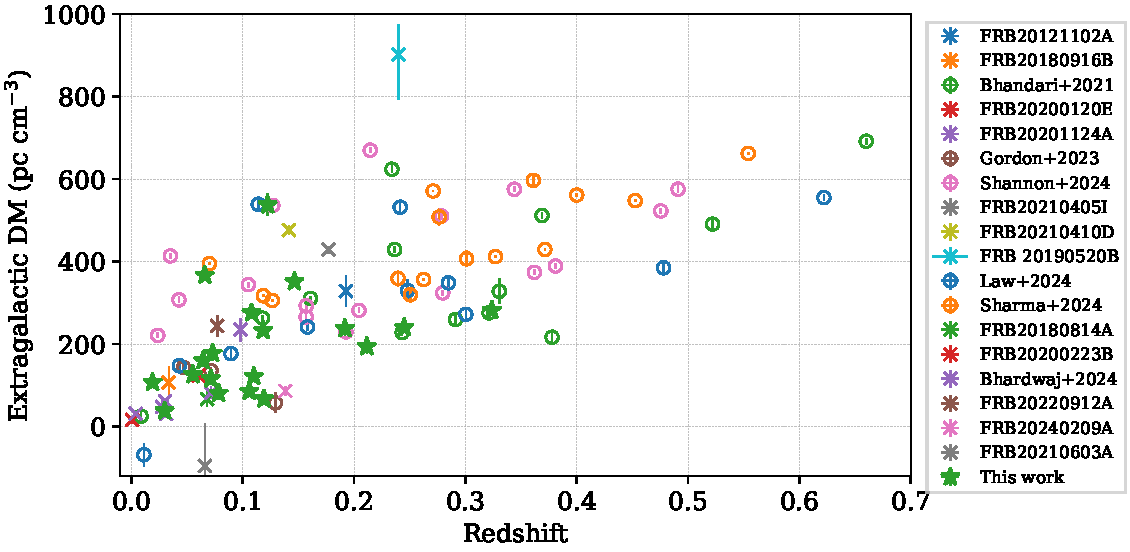
\includegraphics[width=\linewidth]{figures/macquart.pdf}
    \caption{The redshift-FRB dispersion relation for a selection of host galaxies in the literature shows the complementary redshift coverage of various FRB surveys at the time of this writing. Galaxy redshifts and FRB DM measurements are taken from~\citep{bhandari2022characterizing,gordon2023demographics,law2024deep,sharma2024preferential}. Low-DM selected FRBs from CHIME are taken from ~\citet{bhardwaj2021nearby,michilli2023subarcminute,bhardwaj2024host,Ibik2024host}.}
    \label{fig:macquart}
\end{figure*}

\begin{figure*}
    \centering
    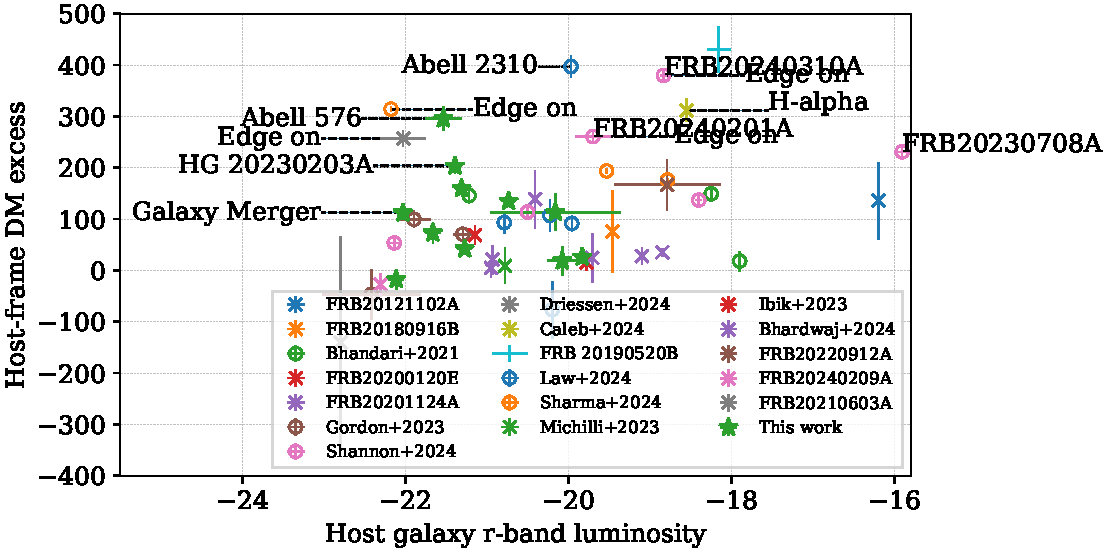
\includegraphics[width=\linewidth]{figures/dm_host.pdf}
    \caption{The DM excess as defined in Eq.~\ref{eq:dmh_definition} after subtracting contributions from the IGM~\citep{macquart2020census}, Milky Way disk~\citep{cordes2002ne2001}, and its halo~\citep{yamasaki2020galactic} as a function of $r$-band host galaxy luminosity for low-redshift FRBs in the literature. Where available we use published dust corrections; otherwise we use published r-band photometry ($i$-band for some sources of~\citet{shannon2024commensal} and J-band for FRB 20190520B) and the~\citet{fitzpatrick2007analysis} model to correct for Galactic extinction. X-axis error bars indicate photometric errors where available, while Y-axis error bars indicate the uncertainty in the NE2001 contribution along that sightline, taken to be $20\%$. The ``Cluster'' and ``Edge on'' labels identify host galaxies associated with known galaxy clusters or highly-inclined host galaxies (see text). The $H\alpha$ label refers to the host galaxy of FRB 20210410D, whose dispersion measure excess can largely -- but not completely -- be attributed to H$\alpha$ emission~\citep{cordes2016radio}.}
    \label{fig:host_dm}
\end{figure*}

The selection effects relevant to this measurement are likely modest. The CHIME/FRB baseband system directly selects against high DM bursts, but this effect is only present when the total DM $> 1000$ pc cm$^{-3}$, and is unlikely to affect our measurement~\citet{collaboration2021first,shin2023inferring}. The CHIME/FRB real-time search pipeline is strongly affected by non-stationary noise, which translates into an lower detection probability for low-flux, highly-scattered bursts. While this could affect the sample of bursts that are detected, we note that bright, highly-scattered bursts are nevertheless detectable~\citep{shin2024investigating}, and that the bursts bright enough to be detected in VLBI should not be strongly subject to this selection effect. We strongly select on host luminosity, because of our localization region, which is usually larger than typical FRB host galaxies. Hence, we caution that our results are only applicable for non-dwarf host galaxies brighter than $M_r < -17$.

%There is a strong selection effect on host redshift, which we don't think should be correlated strongly with DM_h 
% CL: not much of this...
\section{Sensitivity to Cosmic Baryons and Cosmological Parameters}
Here we demonstrate that our measurements are insensitive to galactic feedback. From the estimator in Eq.~\ref{eq:dmh_definition}, we calculate 
$$\dfrac{d(\langle\dmh\rangle)}{d(\Omega_b f_\text{diffuse} H_0)} = \dfrac{XXXX\textrm{pc cm}^{-3}}{0.05 \times 0.7 \times 70 km/s/Mpc}.$$

\section{Comparison to CAMELS}
hi
\section{Conclusion}
We have characterized the mean host contribution of FRB dispersion measures using the largest uniform sample of low-redshift FRBs. We have found that in many cases, the DM excess can be attributed to a nearby galaxy cluster or an edge-on host geometry. We use this additional statistical power to directly measure the enigmatic host galaxy contribution to FRB dispersion measures in a way that is agnostic to any particular parameterization of feedback and fluctuations in the IGM; we measure $\langle\dmh\rangle = 104\pm16$ and $S_h = 113\pm12$ for non-dwarf hosts with $M_r < -17$. Our measurement represents a significant improvement relative to global fitting methods that use a combination of sources at high and low redshifts to break degeneracies under the assumption of a particular redshift evolution of the host galaxy contribution. Model-insensitive measurements of $\dmh$ like the one here will be a crucial anchor for FRB cosmology at higher redshifts, and contain rich information about the spatial distribution of FRBs within their hosts. More broadly, the observational techniques for FRB detection and localization, host galaxy association, and follow-up pave the way for upcoming large-scale FRB surveys~\citep{vanderlinde2019canadian,hallinan2019dsa}, which will revolutionize our understanding of FRBs and the universe they illuminate.

\begin{figure*}
    \centering
    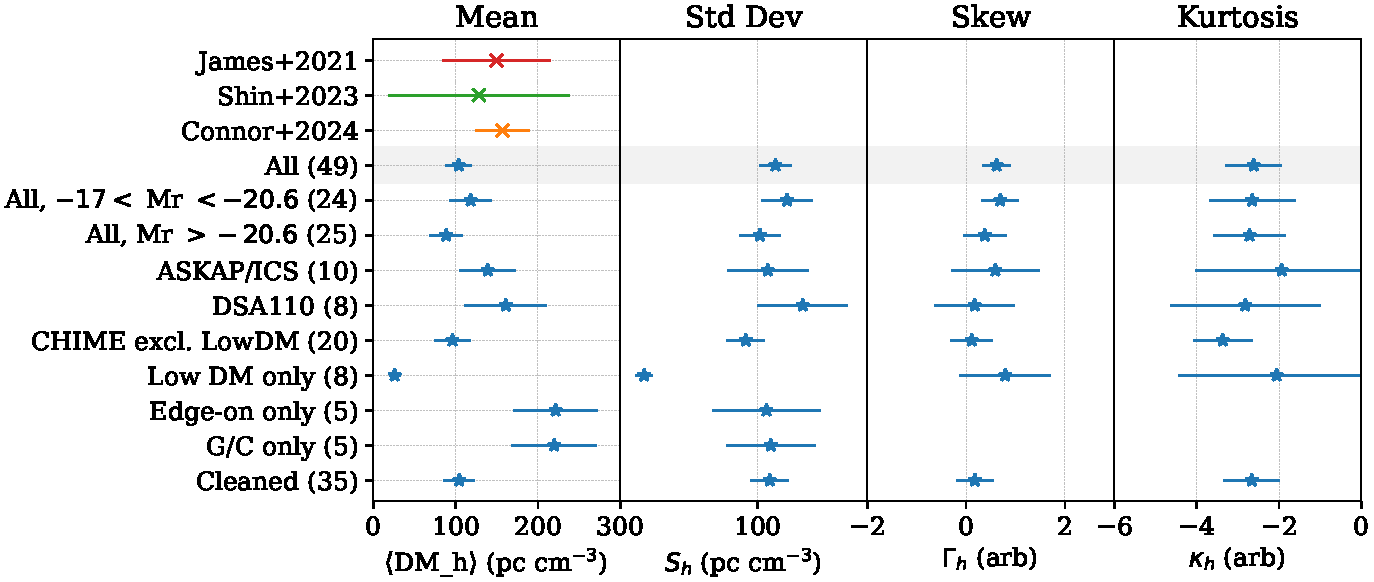
\includegraphics[width=\linewidth]{figures/mvsk.pdf}
    \caption{A graphical representation of Table~\ref{tab:mvsk}, which characterizes the distribution of $\dmh$ using its first four moments. The top three rows show the implied values from global fitting analyses where a log-normal distribution of $\dmh$ is assumed. The shaded grey row denotes the measurement of the \dmh\ distribution using our full sample, which represents the most precise and feedback-insensitive measurement to date.}
    \label{fig:mvsk}
\end{figure*}

\begin{table*}
\caption{Low-redshift estimates of $\langle \dmh\rangle$, $S_h$, $\Gamma_h$,$\kappa_h$ for different subsamples as described in the text. For our measurements, we denote the number of bursts used in each measurement $(N)$, as well as the mean, and standard deviation of the \dmh\ distribution measured in pc cm$^{-3}$, while the skew and excess kurtosis are dimensionless (see text for definitions).}
\begin{tabular}{llllll}
\toprule
 & N & Mean ($\langle\textrm{DM}_h \rangle$) & Std Dev ($S_h$) & Skew ($\Gamma_h$) & Kurtosis ($\kappa_h$) \\
Subsample &  &  &  &  &  \\
\midrule
James+2021 & - & $150 \pm 66$ & $85 \pm 48$ & $1.9 \pm 0.7$ & $7.0 \pm 6.1$ \\
Shin+2023 & - & $128 \pm 110$ & $148 \pm 208$ & - & - \\
Connor+2024 & - & $157 \pm 33$ & $95 \pm 42$ & $2.0 \pm 0.8$ & $8.2 \pm 8.1$ \\
All  & $51$ & $109 \pm 17$ & $115 \pm 12$ & $0.8 \pm 0.3$ & $-2.5 \pm 0.7$ \\
All, $-20.2 < M_r$  & $12$ & $117 \pm 26$ & $87 \pm 18$ & $0.2 \pm 0.7$ & $-2.9 \pm 1.3$ \\
All, $-20.2 > M_r > -21.3$  & $12$ & $117 \pm 26$ & $87 \pm 18$ & $0.2 \pm 0.7$ & $-2.9 \pm 1.3$ \\
All, $M_r < -21.3$  & $11$ & $89 \pm 43$ & $142 \pm 32$ & $0.7 \pm 0.7$ & $-2.5 \pm 1.8$ \\
ASKAP/ICS  & $10$ & $139 \pm 34$ & $107 \pm 29$ & $0.6 \pm 0.9$ & $-1.9 \pm 2.1$ \\
DSA110  & $8$ & $161 \pm 50$ & $133 \pm 33$ & $0.2 \pm 0.8$ & $-2.8 \pm 1.8$ \\
CHIME excl. LowDM  & $22$ & $109 \pm 22$ & $101 \pm 18$ & $0.8 \pm 0.5$ & $-2.3 \pm 1.4$ \\
Low DM only  & $8$ & $26 \pm 7$ & $17 \pm 6$ & $0.8 \pm 0.9$ & $-2.1 \pm 2.4$ \\
Edge-on only  & $5$ & $225 \pm 47$ & $99 \pm 35$ & - & - \\
G/C only  & $5$ & $216 \pm 53$ & $112 \pm 33$ & - & - \\
Cleaned  & $37$ & $111 \pm 19$ & $113 \pm 15$ & $0.5 \pm 0.3$ & $-2.5 \pm 0.7$ \\
\bottomrule
\end{tabular}

\label{tab:mvsk}
\end{table*}
\section{Acknowledgments}
We acknowledge that CHIME and~\kkoname\ are located on the traditional, 
ancestral, and unceded territory of the Syilx/Okanagan people. We are grateful to the staff of the Dominion Radio
Astrophysical Observatory, which is operated by the National Research Council of Canada. 
CHIME is funded by a grant from the Canada Foundation 
for Innovation (CFI) Leading Edge Fund (Project 31170) 
and by contributions from the provinces of British Columbia, 
Qu\'ebec and Ontario. The CHIME/FRB Project is funded by a 
grant from the CFI 2015 Innovation Fund (Project 33213) and 
by contributions from the provinces of British Columbia and 
Qu\'ebec, and by the Dunlap Institute for Astronomy and 
Astrophysics at the University of Toronto. 
Additional support was provided by the Canadian 
Institute for Advanced Research (CIFAR), McGill 
University and the McGill Space Institute via the 
Trottier Family Foundation, and the University of 
British Columbia. 
The CHIME/FRB Outriggers program is funded by 
the Gordon and Betty Moore Foundation and by a National Science Foundation (NSF) grant (2008031).
The \kkoname~Outrigger is situated on land leased from the Imperial Metals Corporation
FRB research at MIT is supported by an NSF grant (2008031).
FRB research at WVU is supported by an NSF grant (2006548, 2018490).

The Pan-STARRS1 Surveys (PS1) and the PS1 public science archive have been made possible through contributions by the Institute for Astronomy, the University of Hawaii, the Pan-STARRS Project Office, the Max-Planck Society and its participating institutes, the Max Planck Institute for Astronomy, Heidelberg and the Max Planck Institute for Extraterrestrial Physics, Garching, The Johns Hopkins University, Durham University, the University of Edinburgh, the Queen's University Belfast, the Harvard-Smithsonian Center for Astrophysics, the Las Cumbres Observatory Global Telescope Network Incorporated, the National Central University of Taiwan, the Space Telescope Science Institute, the National Aeronautics and Space Administration under Grant No. NNX08AR22G issued through the Planetary Science Division of the NASA Science Mission Directorate, the National Science Foundation Grant No. AST-1238877, the University of Maryland, Eotvos Lorand University (ELTE), the Los Alamos National Laboratory, and the Gordon and Betty Moore Foundation.

The Legacy Surveys consist of three individual and complementary projects: the Dark Energy Camera Legacy Survey (DECaLS; Proposal ID \#2014B-0404; PIs: David Schlegel and Arjun Dey), the Beijing-Arizona Sky Survey (BASS; NOAO Prop. ID \#2015A-0801; PIs: Zhou Xu and Xiaohui Fan), and the Mayall z-band Legacy Survey (MzLS; Prop. ID \#2016A-0453; PI: Arjun Dey). DECaLS, BASS and MzLS together include data obtained, respectively, at the Blanco telescope, Cerro Tololo Inter-American Observatory, NSF’s NOIRLab; the Bok telescope, Steward Observatory, University of Arizona; and the Mayall telescope, Kitt Peak National Observatory, NOIRLab. 

Pipeline processing and analyses of the data were supported by NOIRLab and the Lawrence Berkeley National Laboratory (LBNL). The Legacy Surveys project is honored to be permitted to conduct astronomical research on Iolkam Du’ag (Kitt Peak), a mountain with particular significance to the Tohono O’odham Nation.

NOIRLab is operated by the Association of Universities for Research in Astronomy (AURA) under a cooperative agreement with the National Science Foundation. LBNL is managed by the Regents of the University of California under contract to the U.S. Department of Energy.

This project used data obtained with the Dark Energy Camera (DECam), which was constructed by the Dark Energy Survey (DES) collaboration. Funding for the DES Projects has been provided by the U.S. Department of Energy, the U.S. National Science Foundation, the Ministry of Science and Education of Spain, the Science and Technology Facilities Council of the United Kingdom, the Higher Education Funding Council for England, the National Center for Supercomputing Applications at the University of Illinois at Urbana-Champaign, the Kavli Institute of Cosmological Physics at the University of Chicago, Center for Cosmology and Astro-Particle Physics at the Ohio State University, the Mitchell Institute for Fundamental Physics and Astronomy at Texas A\&M University, Financiadora de Estudos e Projetos, Fundacao Carlos Chagas Filho de Amparo, Financiadora de Estudos e Projetos, Fundacao Carlos Chagas Filho de Amparo a Pesquisa do Estado do Rio de Janeiro, Conselho Nacional de Desenvolvimento Cientifico e Tecnologico and the Ministerio da Ciencia, Tecnologia e Inovacao, the Deutsche Forschungsgemeinschaft and the Collaborating Institutions in the Dark Energy Survey. The Collaborating Institutions are Argonne National Laboratory, the University of California at Santa Cruz, the University of Cambridge, Centro de Investigaciones Energeticas, Medioambientales y Tecnologicas-Madrid, the University of Chicago, University College London, the DES-Brazil Consortium, the University of Edinburgh, the Eidgenossische Technische Hochschule (ETH) Zurich, Fermi National Accelerator Laboratory, the University of Illinois at Urbana-Champaign, the Institut de Ciencies de l’Espai (IEEC/CSIC), the Institut de Fisica d’Altes Energies, Lawrence Berkeley National Laboratory, the Ludwig Maximilians Universitat Munchen and the associated Excellence Cluster Universe, the University of Michigan, NSF’s NOIRLab, the University of Nottingham, the Ohio State University, the University of Pennsylvania, the University of Portsmouth, SLAC National Accelerator Laboratory, Stanford University, the University of Sussex, and Texas A\&M University.

BASS is a key project of the Telescope Access Program (TAP), which has been funded by the National Astronomical Observatories of China, the Chinese Academy of Sciences (the Strategic Priority Research Program “The Emergence of Cosmological Structures” Grant \# XDB09000000), and the Special Fund for Astronomy from the Ministry of Finance. The BASS is also supported by the External Cooperation Program of Chinese Academy of Sciences (Grant \# 114A11KYSB20160057), and Chinese National Natural Science Foundation (Grant \# 12120101003, \# 11433005).

The Legacy Survey team makes use of data products from the Near-Earth Object Wide-field Infrared Survey Explorer (NEOWISE), which is a project of the Jet Propulsion Laboratory/California Institute of Technology. NEOWISE is funded by the National Aeronautics and Space Administration.

The Legacy Surveys imaging of the DESI footprint is supported by the Director, Office of Science, Office of High Energy Physics of the U.S. Department of Energy under Contract No. DE-AC02-05CH1123, by the National Energy Research Scientific Computing Center, a DOE Office of Science User Facility under the same contract; and by the U.S. National Science Foundation, Division of Astronomical Sciences under Contract No. AST-0950945 to NOAO.

The Photometric Redshifts for the Legacy Surveys (PRLS) catalog used in this paper was produced thanks to funding from the U.S. Department of Energy Office of Science, Office of High Energy Physics via grant DE-SC0007914.

This work has made use of data from the European Space Agency (ESA) mission
{\it Gaia} (\url{https://www.cosmos.esa.int/gaia}), processed by the {\it Gaia}
Data Processing and Analysis Consortium (DPAC,
\url{https://www.cosmos.esa.int/web/gaia/dpac/consortium}). Funding for the DPAC
has been provided by national institutions, in particular the institutions
participating in the {\it Gaia} Multilateral Agreement.

This research has made use of the CIRADA cutout service at URL cutouts.cirada.ca, operated by the Canadian Initiative for Radio Astronomy Data Analysis (CIRADA). CIRADA is funded by a grant from the Canada Foundation for Innovation 2017 Innovation Fund (Project 35999), as well as by the Provinces of Ontario, British Columbia, Alberta, Manitoba and Quebec, in collaboration with the National Research Council of Canada, the US National Radio Astronomy Observatory and Australia’s Commonwealth Scientific and Industrial Research Organisation. 
\vspace{5mm}
\facilities{CHIME}
\software{\texttt{numpy} \citep{harris2020array}, \texttt{scipy} \citep{virtanen2020scipy}, \texttt{matplotlib}~\citep{hunter2007matplotlib}, 
\texttt{PyFX},\texttt{coda}~\citet{leung2024vlbi},\texttt{difxcalc}~\citet{gordon2016difxcalc}
}
\appendix
\bibliographystyle{aasjournal}
\bibliography{references}



%% This command is needed to show the entire author+affiliation list when
%% the collaboration and author truncation commands are used.  It has to
%% go at the end of the manuscript.
%\allauthors

%% Include this line if you are using the \added, \replaced, \deleted
%% commands to see a summary list of all changes at the end of the article.
%\listofchanges

\end{document}

% End of file `sample631.tex'.